\documentclass{beamer}
\usepackage[utf8]{inputenc}
\usepackage[T1]{fontenc}
\usepackage{subcaption}
\usepackage{wrapfig}
\usepackage[english,polish]{babel}

\graphicspath{ {images/} {images/collisions24x10_2x2} }

\usetheme{CambridgeUS}

\title{Modelowanie elastycznych i nieelastycznych zderzeń obiektów 
metodą dynamiki molekularnej na potrzeby animacji komputerowych}
    \subtitle{ Omówienie tematu pracy magisterskiej }
    \author[Kamil Pasterczyk]{Kamil Pasterczyk \and \\ Promotor: dr hab. inż. Tomasz Chwiej}
    \institute[AGH]{AGH University of Science and Technology}
\date{\today}


\begin{document}

\section{Praca magisterska}
\subsection{Omówienie tematu}

\begin{frame}
    \titlepage
\end{frame}

\begin{frame}
    \frametitle{Cele}

    \begin{block}{MD}
        Jedną z popularnych metod wykorzystywanych w modelowaniu zderzeń obiektów jest
        metoda dynamiki molekularnej. Pierwotnie stosowana do opisu własności gazów i
        cieczy, pozwala również modelować obiekty makroskopowe zachowujące kształt
        oraz modelować ich rozrywanie w trakcie zderzeń z innymi obiektami.
    \end{block}

    W pracy planowane jest opracowanie algorytmów numerycznych do 
    symulacji zderzeń obiektów z możliwością ich rozrywania.
    Implementacja musi być na tyle wydajna aby możliwa była wizualizacja 
     w czasie rzeczywistym jako animacje komputerowe.
\end{frame}

\begin{frame}
    \frametitle{Dlaczego ten temat?}
    \begin{itemize}
        \item Rozinięcie tematu pracy inżynierskiej, nowe możliwości
        \item Przyśpieszenie poprzedniego projektu, optymalizacje
        \item Możliwość rozwinięcia wiedzy odnośnie interesujących mnie technologii
    \end{itemize}
\end{frame}

\begin{frame}
    \frametitle{Wybrane technologie}
    \begin{itemize}
        \item Rust - wybierany jako \emph{most loved programming language} w ankiecie dla programistów
              Stack Overflow w latach 2016, 2017, 2018, 2019, 2020, 2021.
        \item egui - to prosta, szybka i przenośna biblioteka GUI \emph{immediate mode} dla Rust, odpowiednik biblioteki ImGui
        \item OpenGL 4.6 - nie rozwijany ale za to jest nieco przystępniejszy niż Vulkan i bardziej stabilny niż WebGPU.
        \item CUDA, OpenCL - wykorzystywane do przyśpieszenia obliczeń poprzez wykonywania ich części na karcie graficznej
    \end{itemize}
\end{frame}

\begin{frame}
    \frametitle{Model}
    Potencjał Lennarda-Jonesa został wykorzystany do symulacji przyciągania/odpychania węzłów w jednym obiekcie,
    symulacji kolizji węzłów ze ścianami oraz symulacji kolizji węzłów z węzłami należącymi
    do innych obiektów. Wzór na siłę pomiędzy dwoma węzłami wynikającą z potencjału Lennarda-Jonesa wygląda następująco:
    \begin{equation}
        F_{LJ} = 3\frac{V_0}{d_0} \left[ \left(\frac{d_0}{l}\right)^{7} - \left(\frac{d_0}{l}\right)^{13} \right]
    \end{equation}

    Gdzie $l$ to odległość między dwiema oddziałującymi cząstkami, $V_0$ to współczynnik określający wartość potencjału.
    Potencjał Lennarda-Jonesa ma swoje minimum w odległości $d_0$, na tej odległości siła wypadkowa jest zerowa.
\end{frame}

\begin{frame}
    \frametitle{Połączenia międzywęzłowe}

    \begin{figure}[h]
        \begin{subfigure}{0.45\textwidth}
            \centering
            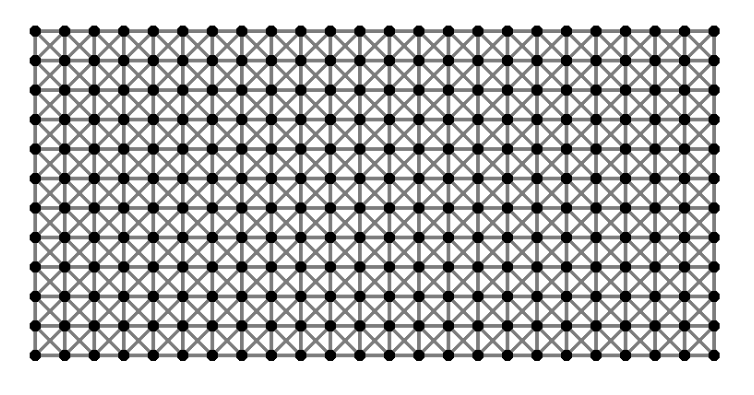
\includegraphics[width=5.5cm]{12x24}
            \caption{Stan początkowy}
        \end{subfigure}
        \begin{subfigure}{0.45\textwidth}
            \centering
            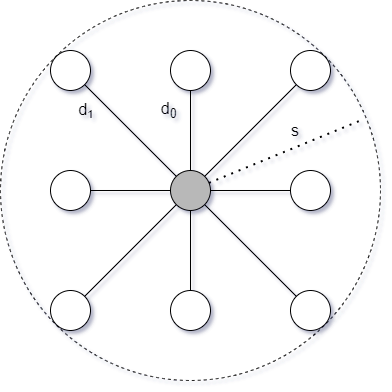
\includegraphics[width=4.5cm]{connections.drawio}
            \caption{Zderzenie}
        \end{subfigure}
    \end{figure}

    Dla każdego węzła znajdujemy wszystkie węzły w odległości $s$, i dodajemy do listy połączeń wraz z informacją
    w jakiej odległości od siebie się znajdują ($d_0$, $d_1$). W ten sposób możemy stworzyć elastyczny obiekt, kształt
    zostanie zachowany.
\end{frame}

\begin{frame}
    \frametitle{Przykład zderzenia - bez zniszczeń}
    \begin{figure}[h]

        \begin{subfigure}{0.4\textwidth}
            \centering
            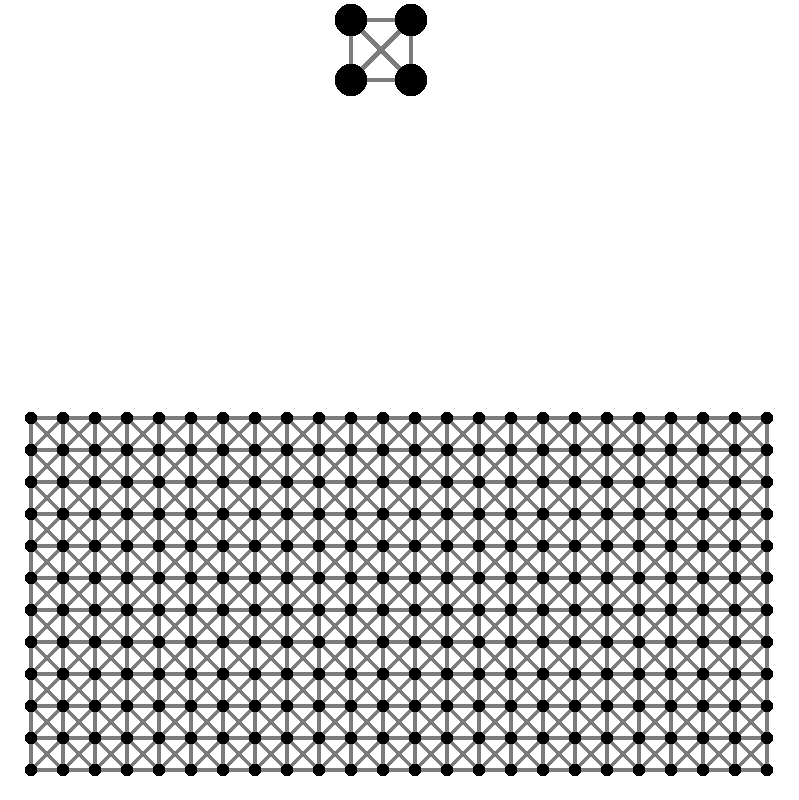
\includegraphics[width=1.7cm, height=1.7cm]{collision_2x2_24x12_mass30_1}
            \caption{Stan początkowy}
        \end{subfigure}
        \begin{subfigure}{0.4\textwidth}
            \centering
            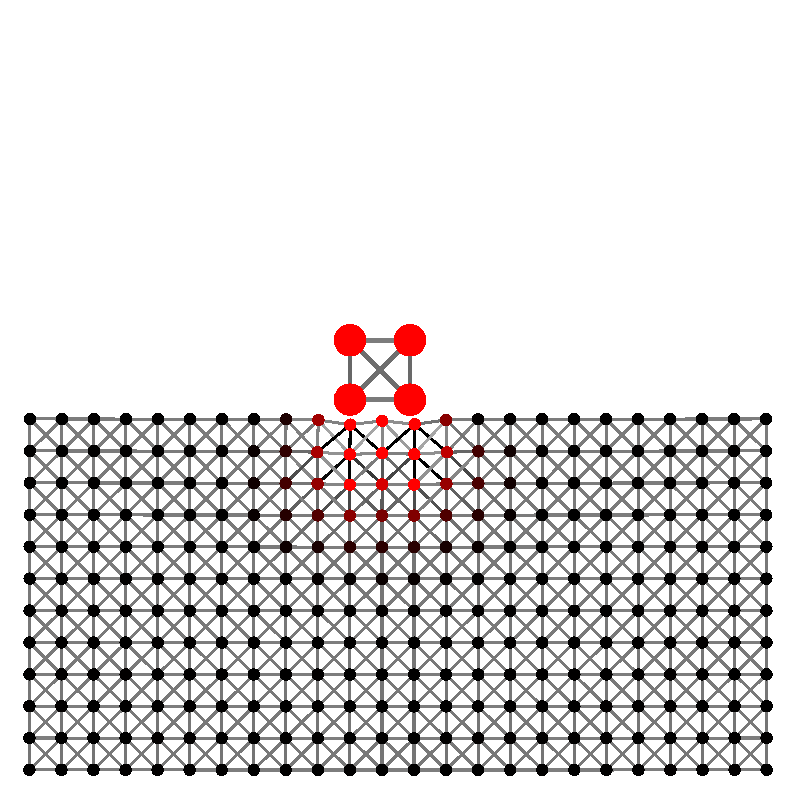
\includegraphics[width=1.7cm, height=1.7cm]{collision_2x2_24x12_mass30_2}
            \caption{Zderzenie}
        \end{subfigure}
        \begin{subfigure}{0.4\textwidth}
            \centering
            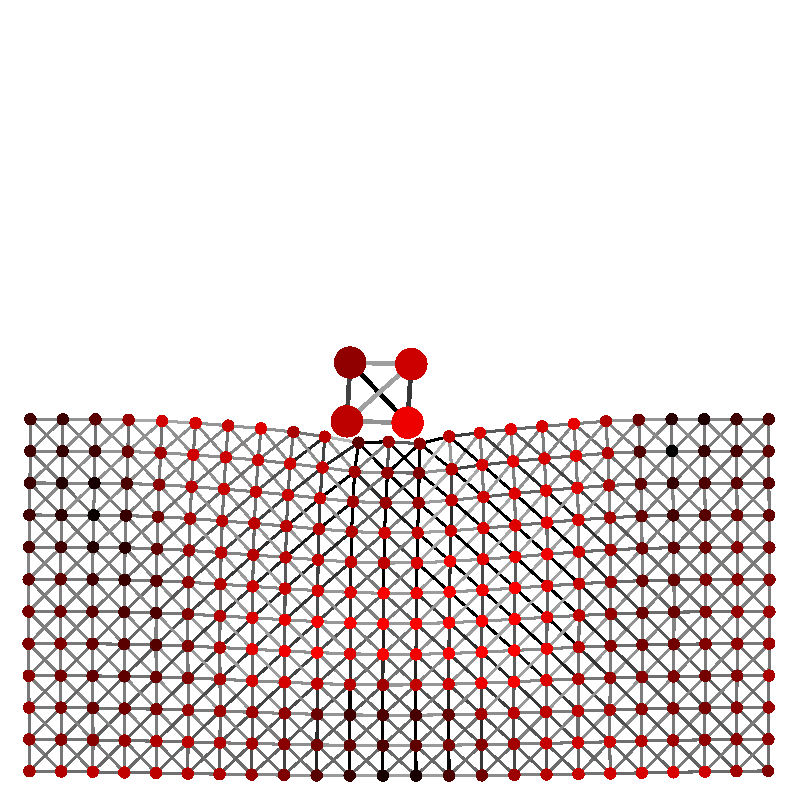
\includegraphics[width=1.7cm, height=1.7cm]{collision_2x2_24x12_mass30_3}
            \caption{Chwila po zderzeniu}
        \end{subfigure}
        \begin{subfigure}{0.4\textwidth}
            \centering
            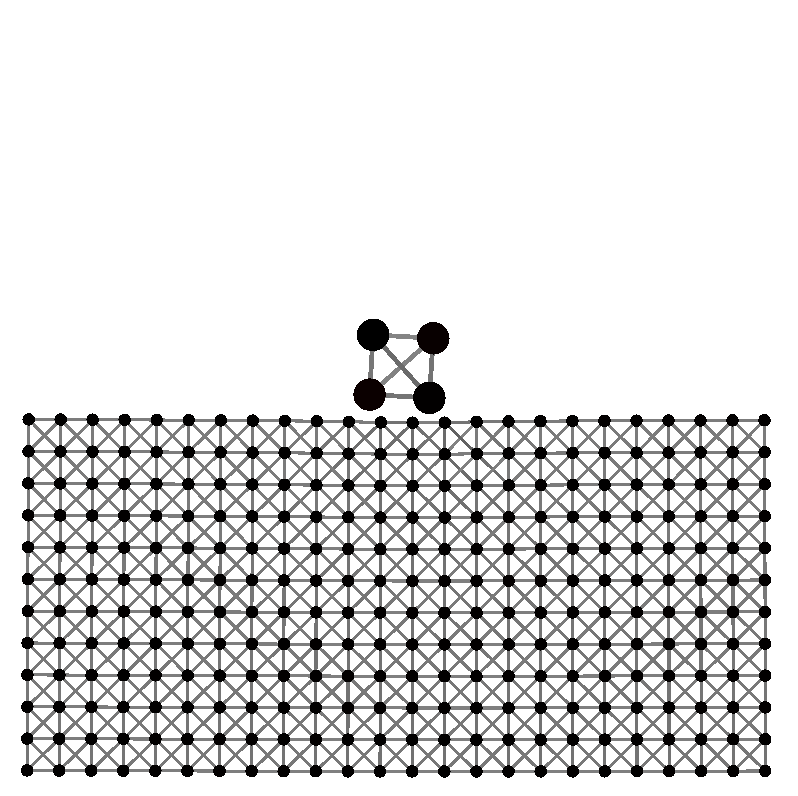
\includegraphics[width=1.7cm, height=1.7cm]{collision_2x2_24x12_mass30_4}
            \caption{Stan stabilny}
        \end{subfigure}

        \caption{Zderzenie spadającego obiektu $2 \times 2$ o masie 120 kg na obiekt $12 \times 24$ o masie 288 kg}
    \end{figure}

    Węzły o kolorze czarnym mają zerową energię kinetyczną, zmienieją kolor na czerwony proporcjonalnie do ilości posiadanej energii kinetczynej.
    Przy zderzeniu widoczny jest transfer energii kinetcznej.
\end{frame}

\begin{frame}
    \frametitle{Przykład zderzenia - rozerwanie obiektów}
    \begin{figure}[h]

        \begin{subfigure}{0.4\textwidth}
            \centering
            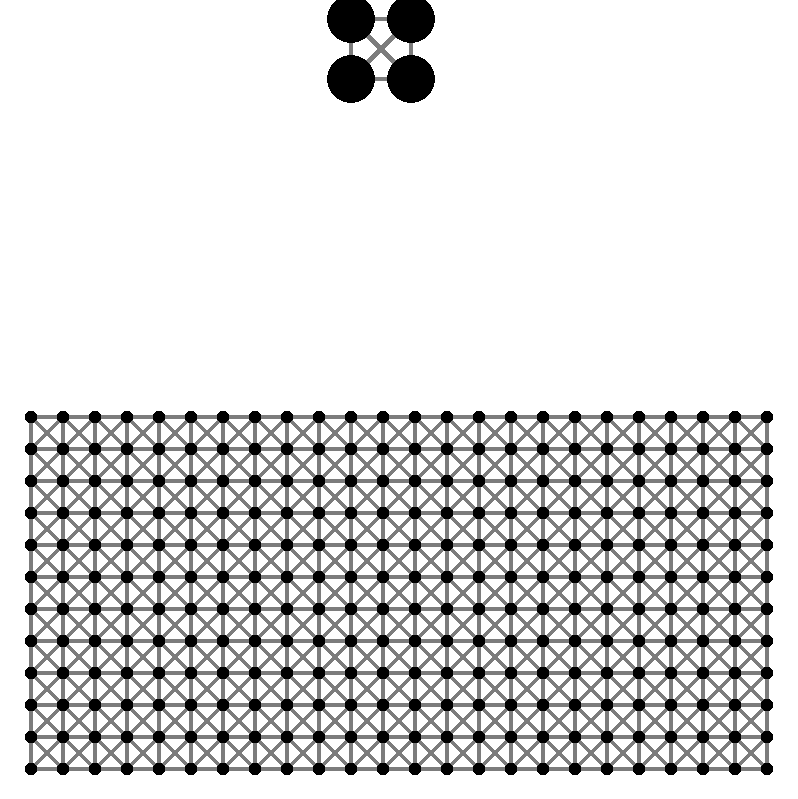
\includegraphics[width=1.7cm, height=1.7cm]{collision_2x2_24x12_mass80_1}
            \caption{Stan początkowy}
        \end{subfigure}
        \begin{subfigure}{0.4\textwidth}
            \centering
            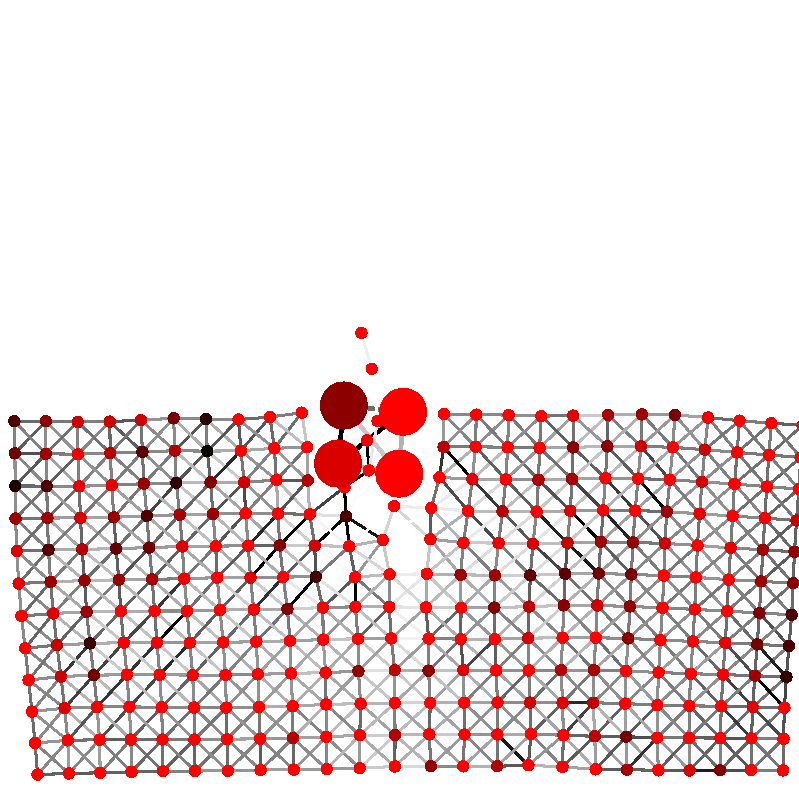
\includegraphics[width=1.7cm, height=1.7cm]{collision_2x2_24x12_mass80_2}
            \caption{Zderzenie}
        \end{subfigure}
        \begin{subfigure}{0.4\textwidth}
            \centering
            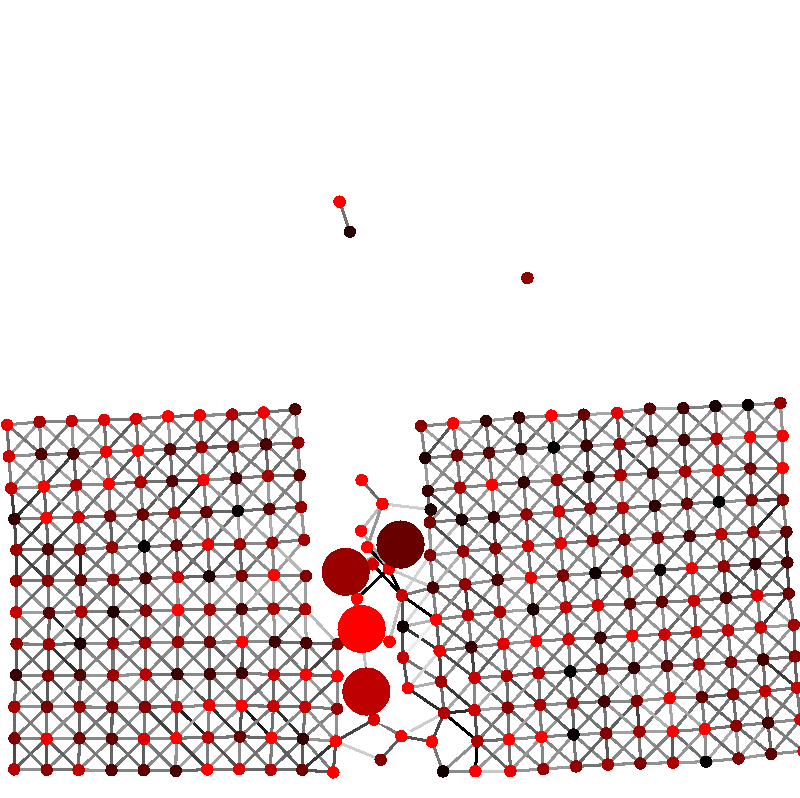
\includegraphics[width=1.7cm, height=1.7cm]{collision_2x2_24x12_mass80_3}
            \caption{Chwila po zderzeniu}
        \end{subfigure}
        \begin{subfigure}{0.4\textwidth}
            \centering
            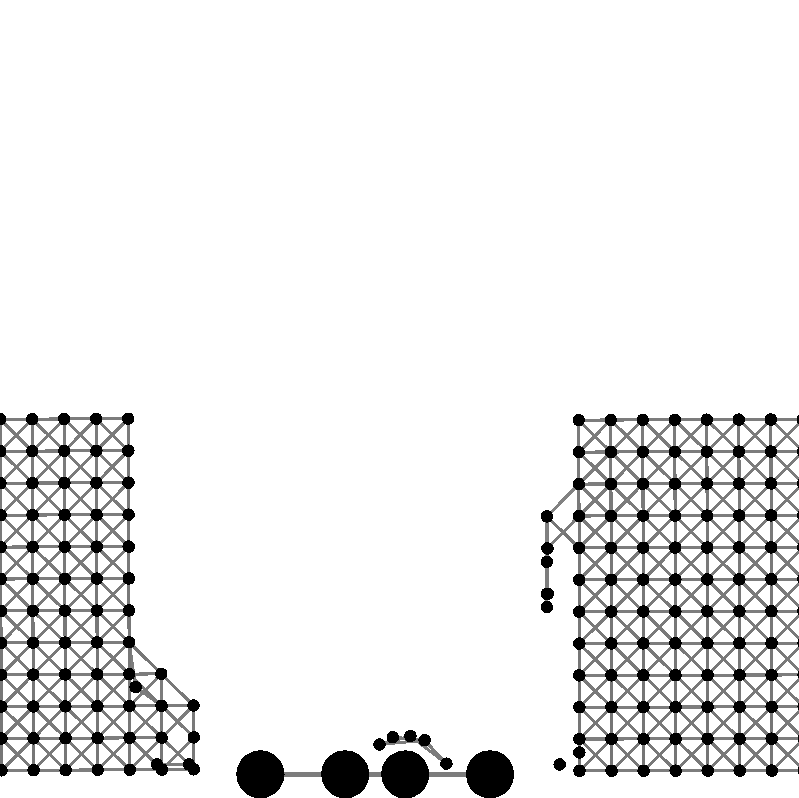
\includegraphics[width=1.7cm, height=1.7cm]{collision_2x2_24x12_mass80_4}
            \caption{Stan stabilny}
        \end{subfigure}

        \caption{Zderzenie spadającego obiektu $2 \times 2$ o masie 320 kg na obiekt $12 \times 24$ o masie 288 kg}
    \end{figure}

    W chwili zderzenia po obiekcie $12 \times 24$ rozchodzi się gwałtownie fala energii kinetycznej a on sam zostaje
    rozerwany, częściowemu zniszczeniu ulega również obiekt $2 \times 2$.
\end{frame}


\begin{frame}
    \frametitle{Optymalizacje i zrównoleglenie}

    Obliczanie kolizji każdy węzłem z każdym węzłem wymaga znacznej ilości czasu - złożoność $O(n^2)$.
    Jednym z głównych celów pracy jest optymalizacja np. sprawdzanie kolizji jedynie węzłów brzegowych.
    Istotne jest również zrównoleglenie procesu obliczania kolizji.
    Jaki będzie wpływ tych optymalizacji na dokładność?

    \begin{block}{Teoria chaosu}
        Efekt motyla przedstawia, w jaki sposób niewielka zmiana w jednym stanie
        deterministycznego układu może skutkować dużymi różnicami w późniejszym stanie.
        Znana anegdota na temat tego efektu mówi że motyl trzepoczący skrzydłami w Brazylii może wywołać tornado w Teksasie.
    \end{block}
\end{frame}

\begin{frame}
    \frametitle{Potencjalne problemy}

    \begin{itemize}
        \item Do symulacji w czasie rzeczywistym potrzebna jest szybka metoda integracji, jak na przykład algorytm prędkościowy Verleta.
              Algortym ten jest jednak mniej dokładny, możliwe anomalie w symulacji.
        \item Potencjał Lennarda Jonesa jest bardzo wrażliwy ze względu na wysokie potęgi, może to prowadzić do
              niestabilności symulacji dla niektórych kombinacji parametrów (masa, wartości potencjału, odległości, prędkość przy zderzeniu itp.).
        \item Zbyt duży krok czasowy również może spowodować niestabilność symulacji, jednak zmniejszenie go zwiększa czas wykonywania.
        \item Koszty zrównoleglenia dla mniejszych układów będą większe niż korzyści,
              należy zbadać dla jakiej ilości węzłow warto obliczać wielowątkowo.
    \end{itemize}
\end{frame}

\begin{frame}
    \frametitle{Co jest jeszcze planowane?}
    \begin{itemize}
        \item Wizualizacja temperatury
        \item Wizualizacja ciśnienia
        \item Testy zachowania energii w układzie bez sił oporu
        \item Porównanie wydajności wersji jendo- i wielowątkowej
        \item Inne optymalizacje, ich wpływ na wydajność i dokładność
    \end{itemize}
\end{frame}


\begin{frame}
    \frametitle{Koniec prezentacji}

    \centering
    \LARGE Dziękuję za uwagę!
\end{frame}

\end{document}